\section{More with Integrals} \label{S:4.7.MoreIntegrals}

\begin{goals}
\item What is the meaning of the definite integral of a rate of change in contexts other than when the rate of change represents velocity?	
\item How can we use definite integrals to measure the area between two curves?
\item How do we decide whether to integrate with respect to $x$ or with respect to $y$ when we try to find the area of a region?
\end{goals} 


%-----------------------------------
% SUBSECTION INTRODUCTION
%-----------------------------------
\subsection*{Introduction}

\begin{marginfigure}[2in] % MARGIN FIGURE
\margingraphics{figures/6_1_Intro.eps} %Picture from active 6.1
\caption{The area between a nonnegative function $f$ and the $x$-axis on the interval $[a,b]$.} \label{F:4.7.Intro}
\end{marginfigure}

Early on in our work with the definite integral, we learned that if we have a nonnegative velocity function, $v$, for an object moving along an axis, the area under the velocity function between $a$ and $b$ tells us the distance the object traveled on that time interval.  Moreover, based on the definition of the definite integral, that area is given precisely by $\int_a^b v(t) \, dt$.  Indeed, for any nonnegative function $f$ on an interval $[a,b]$, we know that $\int_a^b f(x) \, dx$ measures the area bounded by the curve and the $x$-axis between $x = a$ and $x = b$, as shown in Figure~\ref{F:6.1.Intro}.

In this section, we will further explore definite integrals including some important properties of integrals.  In Preview Activity~\ref{PA:6.1}, we begin this investigation by examining the definite integral in different contexts. %% seeing how a single definite integral may be used to represent the area between two curves.

%\begin{marginfigure}[4cm]
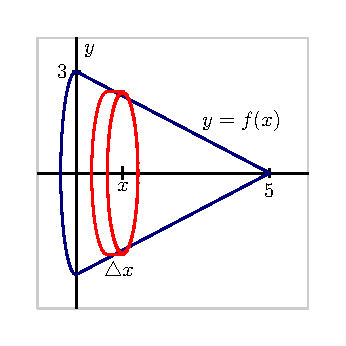
\includegraphics{figures/6_2_PA1.eps}
\caption{The circular cone described in Preview Activity~\ref{PA:6.1}} \label{F:PA.6.1}
\end{marginfigure}


\begin{pa} \label{PA:6.1}  Consider a circular cone of radius $3$ and height $5$, which we view horizontally as pictured in Figure~\ref{F:PA.6.1}.  Our goal in this activity is to use a definite integral to determine the volume of the cone.

\ba
\item Find a formula for the linear function $y = f(x)$ that is pictured in Figure~\ref{F:PA.6.1}.
\item For the representative slice of thickness $\triangle x$ that is located horizontally at a location $x$ (somewhere between $x = 0$ and $x = 5$), what is the radius of the representative slice?  Note that the radius depends on the value of $x$.
\item What is the volume of the representative slice you found in (b)?
\item What definite integral will sum the volumes of the thin slices across the full horizontal span of the cone?  What is the exact value of this definite integral?
\item Compare the result of your work in (d) to the volume of the cone that comes from using the formula $V_{\text{\small{cone}}} = \frac{1}{3} \pi r^2 h.$
\ea
\end{pa} 
\afterpa % PREVIEW ACTIVITY Change activity or the order of the section

%-----------------------------------------------
% SUBSECTION TOTAL CHANGE THEOREM
%-----------------------------------------------

\subsection*{The Total Change Theorem} \index{total change theorem}

As we use the Fundamental Theorem of Calculus to evaluate definite integrals, it is essential that we remember and understand the meaning of the numbers we find.  We briefly summarize three key interpretations to date.
\begin{itemize}
\item For a moving object with instantaneous velocity $v(t)$, the object's change in position on the time interval $[a,b]$ is given by $\int_a^b v(t) \, dt$, and whenever $v(t) \ge 0$ on $[a,b]$, $\int_a^b v(t) \, dt$ tells us the total distance traveled by the object on $[a,b]$.  

\item For any continuous function $f$, its definite integral $\int_a^b f(x) \, dx$ represents the total net signed area bounded by $y = f(x)$ and the $x$-axis on $[a,b]$, where regions that lie below the $x$-axis have a minus sign associated with their area.  

%\item The value of a definite integral is linked to the average value of a function: for a continuous function $f$ on $[a,b]$, its average value $f_{\mbox{\tiny{AVG}}[a,b]}$ is given by
%$$f_{\mbox{\tiny{AVG}}[a,b]} = \frac{1}{b-a} \int_a^b f(x) \, dx.$$
\end{itemize}
%The Fundamental Theorem of Calculus now enables us to evaluate exactly (without taking a limit of Riemann sums) any definite integral for which we are able %to find an antiderivative of the integrand.  

A slight change in notational perspective allows us to gain even more insight into the meaning of the definite integral.  To begin, recall Equation~(\ref{E:FTCV}), where we wrote the Fundamental Theorem of Calculus for a velocity function $v$ with antiderivative $V$ as
\[ V(b) - V(a) = \int_a^b v(t) \ dt. \]
If we instead replace $V$ with $s$ (which represents position) and replace $v$ with $s'$ (since velocity is the derivative of position), Equation~(\ref{E:FTCV}) equivalently reads 
\begin{equation} \label{E:FTCs} % EQUATION
s(b) - s(a) = \int_a^b s'(t) \, dt.
\end{equation}
In words, this version of the FTC tells us that the total change in the object's position function on a particular interval is given by the definite integral of the position function's derivative over that interval.

Of course, this result is not limited to only the setting of position and velocity.  Writing the result in terms of a more general function $f$, we have the Total Change Theorem.

\concept{The Total Change Theorem} % CONCEPT
{If $f$ is a continuously differentiable function on $[a,b]$ with derivative $f'$, then
\begin{equation} \label{E:TotalChange}
f(b) - f(a) = \int_a^b f'(x) \, dx.
\end{equation}
That is, the definite integral of the derivative of a function on $[a,b]$ is the total change of the function itself on $[a,b]$.
} % end concept

The Total Change Theorem tells us more about the relationship between the graph of a function and that of its derivative.  Recall Figure~\ref{F:1.4.ffprime}, which provided one of the first times we saw that heights on the graph of the derivative function come from slopes on the graph of the function itself.  That observation occurred in the context where we knew $f$ and were seeking $f'$; if now instead we think about knowing $f'$ and seeking information about $f$, we can instead say the following:  
\[ \mbox{\emph{differences in heights on $f$ correspond to net signed areas bounded by $f'$.}} \]
\begin{marginfigure} % MARGIN FIGURE
\margingraphics{figures/4_4_TCT.eps}
\caption{The graphs of $f'(x) = 4 - 2x$ (at left) and an antiderivative $f(x) = 4x - x^2$ at right.  Differences in heights on $f$ correspond to net signed areas bounded by $f'$.} \label{F:4.4.TCT}
\end{marginfigure}
To see why this is so, say we consider the difference $f(1) - f(0)$.  Note that this value is 3, in part because $f(1) = 3$ and $f(0) = 0$, but also because the net signed area bounded by $y = f'(x)$ on $[0,1]$ is 3.  That is, $f(1) - f(0) = \int_0^1 f'(x) \, dx$.  A similar pattern holds throughout, including the fact that since the total net signed area bounded by $f'$ on $[0,4]$ is $0$, $\int_0^4 f'(x) \, dx = 0$, so it must be that $f(4) - f(0) = 0$, so $f(4) = f(0)$.

Beyond this general observation about area, the Total Change Theorem enables us to consider interesting and important problems where we know the rate of change, and answer key questions about the function whose rate of change we know.

%\begin{marginfigure} % MARGIN FIGURE
\margingraphics{figures/4_4_TCTEx.eps}
\caption{The rate $r(t)$ of pollution leaking from a tank, measured in gallons per day.} \label{F:4.4.TCTEx}
\end{marginfigure} 

\begin{example} \label{eg:4.7.1} % EXAMPLE
Suppose that pollutants are leaking out of an underground storage tank at a rate of $r(t)$ gallons/day, where $t$ is measured in days.  It is conjectured that $r(t)$ is given by the formula $r(t) = 0.0069t^3 -0.125t^2+11.079$ over a certain 12-day period.  The graph of $y=r(t)$ is given in Figure~\ref{F:4.4.TCTEx}.  What is the meaning of $\int_4^{10} r(t) \, dt$ and what is its value?  What is the average rate at which pollutants are leaving the tank on the time interval $4 \le t \le 10$?

\solution We know that since $r(t) \ge 0$, the value of $\int_4^{10} r(t) \, dt$ is the area under the curve on the interval $[4,10]$.  If we think about this area from the perspective of a Riemann sum, the rectangles will have heights measured in gallons per day and widths measured in days, thus the area of each rectangle will have units of
\[ \frac{\mbox{gallons}}{\mbox{day}} \cdot \mbox{days} = \mbox{gallons}. \]
Thus, the definite integral tells us the total number of gallons of pollutant that leak from the tank from day 4 to day 10.  The Total Change Theorem tells us the same thing:  if we let $R(t)$ denote the function that measures the total number of gallons of pollutant that have leaked from the tank up to day $t$, then $R'(t) = r(t)$, and 
\[ \int_4^{10} r(t) \, dt = R(10) - R(4), \]
which is the total change in the function that measures total gallons leaked over time, thus the number of gallons that have leaked from day 4 to day 10.

To compute the exact value, we use the Fundamental Theorem of Calculus.  Antidifferentiating $r(t) = 0.0069t^3 -0.125t^2+11.079$, we find that
\begin{eqnarray*}
\int_4^{10} (0.0069t^3 -0.125t^2+11.079) \, dt & = & \left. \left( 0.0069 \cdot \frac{1}{4} \, t^4 - 0.125 \cdot \frac{1}{3} t^3 + 11.079t \right) \right|_4^{10} \\
& = & \left( 0.0069 \cdot \frac{1}{4} \, (10)^4 - 0.125 \cdot \frac{1}{3} (10)^3 + 11.079(10) \right) - \\
& \ &  \left( 0.0069 \cdot \frac{1}{4} \, (4)^4 - 0.125 \cdot \frac{1}{3} (4)^3 + 11.079(4) \right) \\
& \approx & 44.282. 
\end{eqnarray*}
Thus, approximately 44.282 gallons of pollutant leaked over the six day time period.

To find the average rate at which pollutant leaked from the tank over $4 \le t \le 10$, we want to compute the average value of $r$ on $[4,10]$.  Thus,
\[ r_{\mbox{\tiny{AVG}}[4,10]} = \frac{1}{10-4} \int_4^{10} r(t) \ dt \approx \frac{44.282}{6} = 7.380, \]
which has its units measured in gallons per day.
\end{example} % EXAMPLE

%\begin{activity} \label{A:4.4.3}  During a 30-minute workout, a person riding an exercise machine burns calories at a rate of $c$ calories per minute, where the function $y = c(t)$ is given in Figure~\ref{F:4.4.Act3}.  On the interval $0 \le t \le 10$, the formula for $c$ is $c(t) = -0.05t^2 + t + 10$, while on $20 \le t \le 30$, its formula is $c(t) = -0.05t^2 + 2t - 5$.
\begin{figure}[h]
\begin{center}
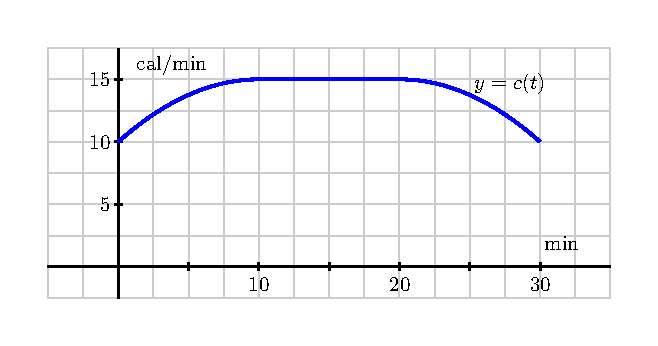
\includegraphics{figures/4_4_Act3.eps}
\caption{The rate $c(t)$ at which a person exercising burns calories, measured in calories per minute.} \label{F:4.4.Act3}
\end{center}
\end{figure}
\ba
	\item What is the exact total number of calories the person burns during the first 10 minutes of her workout?
	\item Let $C(t)$ be an antiderivative of $c(t)$.  What is the meaning of $C(30) - C(0)$ in the context of the person exercising?  Include units on your answer.
	\item Determine the exact average rate at which the person burned calories during the 30-minute workout.
	\item At what time(s), if any, is the instantaneous rate at which the person is burning calories equal to the average rate at which she burns calories, on the time interval $0 \le t \le 30$?
\ea
\end{activity}
\begin{smallhint}
\ba
	\item What are the units on the area of a rectangle found in a Riemann sum for the function $y= c(t)$?
	\item Use the FTC.
	\item Recall the formula for $c_{\mbox{\tiny{AVG}}[0,30]}$.
	\item Think carefully about which function tells you the instantaneous rate at which calories are burned.
\ea
\end{smallhint}
\begin{bighint}
\ba
	\item What are the units on the area of a rectangle found in a Riemann sum for the function $y= c(t)$?  What will be the units on area bounded by the curve?
	\item Use a definite integral and the FTC, as well as your work in (a).
	\item Recall the formula for $c_{\mbox{\tiny{AVG}}[0,30]}$.  Think about the relevant integral in terms of three subintervals: $[0,10]$, $[10,20]$, and $[20,30]$.
	\item Think carefully about which function tells you the instantaneous rate at which calories are burned, and consider your result in (c).
\ea
\end{bighint}
\begin{activitySolution}
\ba
	\item Since the units on a rectangle in a Riemann sum are cal/min for the height and min for the width, the units on the area of such a rectangle are calories, and hence the units on area under the curve $y = c(t)$ are given in total calories.  Hence, the total calories burned during the first 10 minutes of the workout is given by the definite integral $\int_0^{10} c(t) \, dt$.  We use the FTC and evaluate the integral, finding that
	\begin{eqnarray*}
		\int_0^{10} (-0.05t^2 + t + 10) \, dt & = & \left. \left( -\frac{0.05}{3} t^3 + \frac{1}{2} t^2 + 10t \right) \right|_0^{10} \\
				& = &  \left( -\frac{0.05}{3} (10)^3 + \frac{1}{2} (10)^2 + 10(10) \right) - (-0 + 0 + 0) \\
				& = & \frac{400}{3} \ \mbox{calories}.
	\end{eqnarray*}
	Thus, the person burned approximately 133.33 calories in the first 10 minutes of the workout.
	\item We observe first that by the Total Change Theorem, $C(30) - C(0) = \int_0^{30} C'(t) \, dt = \int_0^{30} c(t) \, dt$, and therefore, as discussed in (a), the meaning of this value is the total calories burned on $[0,30]$.
	\item The exact average rate at which the person burned calories on $0 \le t \le 30$ is given by 
	$$c_{\mbox{\tiny{AVG}}[0,30]} = \frac{1}{30-0} \int_0^{30} c(t) \, dt.$$
	To calculate $\int_0^{30} c(t) \, dt,$ we recognize that $c(t)$ is defined in piecewise fashion, and use the additive property of the definite integral, which tells us that 
	$$\int_0^{30} c(t) \, dt = \int_0^{10} c(t) \, dt +  \int_{10}^{20} c(t) \, dt +  \int_{20}^{30} c(t) \, dt.$$
	We know from our work in (a) that $\int_0^{10} c(t) \, dt = \frac{400}{3}$.  Since $c(t) = 15$ is constant on $10 \le t \le 20$, it follows that $ \int_{10}^{20} c(t) \, dt  = 15 \cdot 10 = 150$.  And finally, it is straightforward to show using $c(t) = -0.05t^2 + 2t - 5$ on $20 \le t \le 30$ that $\int_{20}^{30} c(t) \, dt = \frac{400}{3}$.  Hence,
	\begin{eqnarray*}
	\int_0^{30} c(t) \, dt & = & \int_0^{10} c(t) \, dt +  \int_{10}^{20} c(t) \, dt +  \int_{20}^{30} c(t) \, dt \\
			& = & \frac{400}{3} + 150 + \frac{400}{3} \\
			& = & \frac{1250}{3} \approx 416.67 \ \mbox{calories}.
	\end{eqnarray*}
	Now, it follows that the exact average rate at which calories were burned on $[0,30]$ is
	$$c_{\mbox{\tiny{AVG}}[0,30]} = \frac{1}{30-0} \int_0^{30} c(t) \, dt = \frac{1}{30} \cdot \frac{1250}{3} = \frac{1250}{90} \approx 13.89 \ \mbox{cal/min}.$$
	\item It makes sense intuitively that there must be at least one time at which the instantaneous rate at which calories are burned equals the average rate at which calories are burned, as it would be impossible for a continuous instantaneous rate of change to always be above its average value.  Since we know from (c) that $c_{\mbox{\tiny{AVG}}[0,30]} = \frac{125}{9}$, and $c(t)$ tells us the instantaneous rate at which calories are burned, it follows that we want to solve the equation
	$$c(t) = \frac{125}{9}.$$
From the graph, it appears that there are two such values of $t$ for which this equation is true, one in the first ten minutes, and one in the last ten.  For instance, solving
$$-0.05t^2 + t + 10 = \frac{125}{9},$$
it follows that $t = 10 \pm 10\sqrt{2}/3 \approx 14.714, 5.286$, only the second of which lies in $0 \le t \le 10$.  So one time at which the instantaneous rate at which calories are burned equals the average rate on $[0,30]$ is $t = 10 - 10\sqrt{2}/3 \approx 5.286.$  Similar reasoning shows that the other time is $t = 20 + 10\sqrt{2}/3 \approx 24.714$.
\ea
\end{activitySolution}
\aftera





 % ACTIVITY

%----------------------------------------------------
% SUBSECTION AREA BETWEEN TWO CURVES
%----------------------------------------------------

\subsection*{The Area Between Two Curves} \index{area}

Through Preview Activity~\ref{PA:6.1}, we encounter a natural way to think about the area between two curves:  the area between the curves is the area beneath the upper curve minus the area below the lower curve.    For the functions $f(x) = (x-1)^2 + 1$ and $g(x) = x+2$, shown in Figure~\ref{F:6.1.PA1revisited}, 
\begin{marginfigure} % MARGIN FIGURE
\margingraphics{figures/6_1_PA1revisited.eps}
\caption{The areas bounded by the functions $f(x) = (x-1)^2 + 1$ and $g(x) = x+2$ on the interval $[0,3]$.} \label{F:6.1.PA1revisited}
\end{marginfigure}
we see that the upper curve is $g(x) = x+2$, and that the graphs intersect at $(0,2)$ and $(3,5)$.  Note that we can find these intersection points by solving the system of equations given by $y = (x-1)^2 + 1$ and $y = x+2$ through substitution:  substituting $x+2$ for $y$ in the first equation yields $x+2 = (x-1)^2 + 1$, so $x+2 = x^2 - 2x + 1 + 1$, and thus
\[ x^2 - 3x = x(x-3) = 0, \]
from which it follows that $x = 0$ or $x = 3$.  Using $y = x+2$, we find the corresponding $y$-values of the intersection points.

On the interval $[0,3]$, the area beneath $g$ is
\[ \int_0^3 (x+2) \, dx = \frac{21}{2}, \]
while the area under $f$ on the same interval is
\[ \int_0^3 [(x-1)^2 + 1] \, dx = 6. \]
Thus, the area between the curves is 
\begin{equation} \label{E:DiffOfInt} % EQUATION
A = \int_0^3 (x+2) \, dx -  \int_0^3 [(x-1)^2 + 1] \, dx = \frac{21}{2} - 6 = \frac{9}{2}.
\end{equation}

A slightly different perspective is also helpful here:  if we take the region between two curves and slice it up into thin vertical rectangles (in the same spirit as we originally sliced the region between a single curve and the $x$-axis in Section~\ref{S:4.2.Riemann}), then we see that the height of a typical rectangle is given by the difference between the two functions.  For example, for the rectangle shown at left in Figure~\ref{F:6.1.PA1revisited2}, 

\begin{marginfigure} % MARGIN FIGURE
\margingraphics{figures/6_1_PA1revisited2.eps}
\caption{The area bounded by the functions $f(x) = (x-1)^2 + 1$ and $g(x) = x+2$ on the interval $[0,3]$.} \label{F:6.1.PA1revisited2}
\end{marginfigure}

we see that the rectangle's height is $g(x) - f(x)$, while its width can be viewed as $\triangle x$, and thus the area of the rectangle is
\[ A_{\mbox{\small{rect}}} = (g(x) - f(x)) \triangle x. \]
In addition, the area between the two curves on the interval $[0,3]$ is then approximated by the Riemann sum
\[ A \approx \sum_{i=1}^{n} (g(x_i) - f(x_i)) \triangle x, \]
and then as we let $n \to \infty$, it follows that the area is given by the single definite integral
\begin{equation} \label{E:IntOfDiff} % EQUATION 
A = \int_0^3 (g(x) - f(x)) \, dx.
\end{equation}
In our work with applications of the definite integral, we will often find it helpful to think of a ``representative slice'' and how the definite integral may be used to add these slices to find the exact value of a desired quantity.  Here, the integral essentially sums the areas of thin rectangles.

Finally, we note that whether we think of the area between two curves as stemming from the difference between the area bounded by the individual curves (as in Equation~(\ref{E:DiffOfInt})) or as the limit of a Riemann sum that adds the areas of thin rectangles between the curves (as in Equation~(\ref{E:IntOfDiff})), these two results are the same, since the difference of two integrals is the integral of the difference:
\[ \int_0^3 g(x) \, dx -  \int_0^3 f(x) \ dx = \int_0^3 (g(x) - f(x)) \ dx. \]

Moreover, our work so far in this section exemplifies the following general principle.

\concept{} % CONCEPT 
{ If two curves $y = g(x)$ and $y = f(x)$ intersect at $(a,g(a))$ and $(b,g(b))$, and for all $x$ such that $a \le x \le b$, $g(x) \ge f(x)$, then the area between the curves is 
$$A = \int_a^b (g(x) - f(x)) \, dx.$$
} % end concept

%\begin{example} % EXAMPLE
Find the area of the region bounded by $y=x^2+x-5$ and $y=3x-2$.

\solution We begin by finding the $x$-values at which the functions intersect. 
\begin{align*} x^2+x-5 &= 3x-2 \\
(x^2+x-5) - (3x-2) &= 0\\
x^2-2x-3 &= 0\\
(x-3)(x+1) &= 0\\
x&=-1,\ 3.
\end{align*}
Therefore, the area is 
\begin{align*}
\int_{-1}^3\big(3x-2 -(x^2+x-5)\big)\ dx &= \int_{-1}^3 (-x^2+2x+3)\ dx \\
&=\left.\left(-\frac13x^3+x^2+3x\right)\right|_{-1}^3 \\
&=-\frac{27}{3}+9+9-\left(\frac13+1-3\right)\\
&= \frac{32}{3}.
\end{align*}
\end{example} % EXAMPLE

%\begin{activity} \label{A:6.1.1}  
In each of the following questions, draw a careful, labeled sketch of the region described, as well as the solid that results from revolving the region about the stated axis.  In addition, draw a representative slice and state the volume of that slice, along with a definite integral whose value is the volume of the entire solid.  
\ba
\item The region $S$ bounded by the $x$-axis, the curve $y = \sqrt{x}$, and the line $x = 4$; revolve $S$ about the $x$-axis.
\item The region $S$ bounded by the $x$-axis, the curve $y = \sqrt{x}$, and the line $y = 2$; revolve $S$ about the $x$-axis.
\item The finite region $S$ in the first quadrant bounded by the curves $y = \sqrt{x}$ and $y = x^3$; revolve $S$ about the $x$-axis.
\item The finite region $S$ bounded by the curves $y = 2x^2 + 1$ and $y  = x^2 + 4$; revolve $S$ about the $x$-axis.
\item The region $S$ bounded by the $y$-axis, the curve $y = \sqrt{x}$, and the line $y=2$; revolve $S$ about the $y$-axis.  How does the problem change when we revolve about the $y$-axis?
\ea

\end{activity}
\begin{smallhint}
\ba
	\item Small hints for each of the prompts above.
\ea
\end{smallhint}
\begin{bighint}
\ba
	\item Big hints for each of the prompts above.
\ea
\end{bighint}
\begin{activitySolution}
\ba
	\item Solutions for each of the prompts above.
\ea
\end{activitySolution}
\aftera
 % ACTIVITY

%---------------------------------------------------------------
% SUBSECTION MEAN VALUE THEOREM FOR INTEGRALS
%---------------------------------------------------------------

\subsection*{The Average Value of a Function}\index{average value of a function}

One of the most valuable applications of the definite integral is that it provides a way to meaningfully discuss the average value of a function, even for a function that takes on infinitely many values.  Suppose we wish to take the average of $n$ numbers $y_1$, $y_2$, $\ldots$, $y_n$.  We do so by computing
\[ \mbox{Avg} = \frac{y_1 + y_2 + \cdots + y_n}{n}. \]

Since integrals arise from Riemann sums in which we add $n$ values of a function, it should not be surprising that evaluating an integral is something like averaging the output values of a function.  Consider, for instance, the right Riemann sum $R_n$ of a function $f$, which is given by
\begin{align*}
R_n & = f(x_1) \triangle x + f(x_2) \triangle x + \cdots + f(x_n) \triangle x \\
& = (f(x_1) + f(x_2) + \cdots + f(x_n))\triangle x.
\end{align*}
Since $\triangle x = \frac{b-a}{n}$, we can thus write 
\begin{align} \label{E:RAvg}
R_n &  = (f(x_1) + f(x_2) + \cdots + f(x_n))\cdot \frac{b-a}{n} \notag \\
& = (b-a) \frac{f(x_1) + f(x_2) + \cdots + f(x_n)}{n}.
\end{align}
Here, we see that the right Riemann sum with $n$ subintervals is the length of the interval $(b-a)$ times the average of the $n$ function values found at the right endpoints.  And just as with our efforts to compute area, we see that the larger the value of $n$ we use, the more accurate our average of the values of $f$ will be.  Indeed, we will define the average value of $f$ on $[a,b]$ to be 
\[ f_{\mbox{\tiny{AVG}}[a,b]} = \lim_{n \to \infty} \frac{f(x_1) + f(x_2) + \cdots + f(x_n)}{n}.\]  
But we also know that for any continuous function $f$ on $[a,b]$, taking the limit of a Riemann sum leads precisely to the definite integral.  That is, $\ds \lim_{n \to \infty} R_n = \int_a^b f(x) \, dx$, and thus taking the limit as $n \to \infty$ in Equation~(\ref{E:RAvg}), we have that
\begin{equation} \label{E:RAvg2} % EQUATION
\int_a^b f(x) \, dx = (b-a) \cdot f_{\mbox{\tiny{AVG}}[a,b]}.
\end{equation}
Solving Equation~(\ref{E:RAvg2}) for $f_{\mbox{\tiny{AVG}}[a,b]}$, we have the following general principle.

\concept{Average value of a function} % CONCEPT
{If $f$ is a continuous function on $[a,b]$, then its average value on $[a,b]$ is given by the formula
\[ f_{\mbox{\tiny{AVG}}[a,b]} = \frac{1}{b-a} \cdot \int_a^b f(x) \, dx. \]
} % end concept

Observe that Equation~(\ref{E:RAvg2}) tells us another way to interpret the definite integral:  the definite integral of a function $f$ from $a$ to $b$ is the length of the interval $(b-a)$ times the average value of the function on the interval.  In addition, Equation~(\ref{E:RAvg2}) has a natural visual interpretation when the function $f$ is nonnegative on $[a,b]$.  
\begin{marginfigure} % MARGIN FIGURE
\margingraphics{figures/4_3_AvgVal.eps}
\caption{A function $y = f(x)$, the area it bounds, and its average value on $[a,b]$.} \label{F:4.3.AvgVal}
\end{marginfigure}
Consider Figure~\ref{F:4.3.AvgVal}, where we see at left the shaded region whose area is $\int_a^b f(x) \, dx$, at center the shaded rectangle whose dimensions are $(b-a)$ by $f_{\mbox{\tiny{AVG}}[a,b]}$, and at right these two figures superimposed.  Specifically, note that in dark green we show the horizontal line $y = f_{\mbox{\tiny{AVG}}[a,b]}$.  Thus, the area of the green rectangle is given by $(b-a) \cdot f_{\mbox{\tiny{AVG}}[a,b]}$, which is precisely the value of $\int_a^b f(x) \, dx$.  Said differently, the area of the blue region in the left figure is the same as that of the green rectangle in the center figure; this can also be seen by observing that the areas $A_1$ and $A_2$ in the rightmost figure appear to be equal.  Ultimately, the average value of a function enables us to construct a rectangle whose area is the same as the value of the definite integral of the function on the interval.  The java applet\footnote{David Austin, \href{http://gvsu.edu/s/5r}{\texttt{http://gvsu.edu/s/5r}}.} at \href{http://gvsu.edu/s/az}{\texttt{http://gvsu.edu/s/az}} provides an opportunity to explore how the average value of the function changes as the interval changes, through an image similar to that found in Figure~\ref{F:4.3.AvgVal}.

\begin{activity} \label{A:4.7.av}  Suppose that $\ds v(t) = \sqrt{4-(t-2)^2}$ tells us the instantaneous velocity of a moving object on the interval $0 \le t \le 4$, where $t$ is measured in minutes and $v$ is measured in meters per minute.
\ba
\item Sketch an accurate graph of $y = v(t)$.  What kind of curve is $\ds y = \sqrt{4-(t-2)^2}$?
\item Evaluate $\ds \int_0^4 v(t) \, dt$.
\item In terms of the physical problem of the moving object with velocity $v(t)$, what is the meaning of $\ds \int_0^4 v(t) \, dt$?  Include units on your answer.
\item Determine the exact average value of $v(t)$ on $[0,4]$.  Include units on your answer.
\item Sketch a rectangle whose base is the line segment from $t=0$ to $t = 4$ on the $t$-axis such that the rectangle's area is equal to the value of $\ds \int_0^4 v(t) \, dt$.  What is the rectangle's exact height?
\item How can you use the average value you found in (d) to compute the total distance traveled by the moving object over $[0,4]$?
\ea
\end{activity}
\begin{smallhint}
\ba
	\item Note that $y = \sqrt{4-(t-2)^2}$ is part of the curve given by $(t-2)^2 + y^2 = 4$.
	\item What familiar shape is generated by the curve $y = v(t)$?
	\item Recall the meaning of the area bounded by a nonnegative velocity function on a given interval.
	\item From the meaning of the average value of a function, we know $v_{\mbox{\tiny{AVG}}}[a,b] = \frac{1}{b-a}  \int_a^b v(t) \, dt$.
	\item Consider a key recent figure in the text.
	\item Distance equals average rate times $\ldots$.
\ea
\end{smallhint}
\begin{bighint}
\ba
	\item Note that $y = \sqrt{4-(t-2)^2}$ is the top half of the curve given by $(t-2)^2 + y^2 = 4$, which is a familiar one.
	\item What familiar shape is generated by the curve $y = v(t)$?  What known formula for area helps?
	\item Recall the meaning of the area bounded by a nonnegative velocity function on a given interval.  See, for instance, Section~\ref{S:4.1.VelocityDistance}.
	\item From the meaning of the average value of a function, we know $v_{\mbox{\tiny{AVG}}}[a,b] = \frac{1}{b-a}  \int_a^b v(t) \, dt$.  What are $a$ and $b$ in this problem?
	\item Consider a key recent figure in the text and construct a similar drawing for the given function $v$.
	\item Distance equals average rate times time!
\ea
\end{bighint}
\begin{activitySolution}
\ba
	\item The curve $y = v(t) = \sqrt{4-(t-2)^2}$ is the top half of the circle $(t-2)^2 + y^2 = 4$, which has radius 2 and is centered at $(2,0)$.
	\item Thus, the value of $\int_0^4 v(t) \, dt$ is the area of a semicircle of radius 2, which is $\frac{1}{2} \pi (2)^2 = 2\pi$.
	\item Because the velocity $v(t)$ is always nonnegative in this problem, the meaning of $\int_0^4 v(t) \, dt = 2\pi$ is both the distance traveled and the change in position of the object on the interval $0 \le t \le \pi$.  Specifically, the object moved $2 \pi$ meters in 4 minutes.
	\item We know $v_{\mbox{\tiny{AVG}}}[a,b] = \frac{1}{b-a}  \int_a^b v(t) \, dt$, so
	$$v_{\mbox{\tiny{AVG}}}[0,4] = \frac{1}{4-0}  \int_0^4 \sqrt{4-(t-2)^2} \, dt = \frac{1}{4} 2\pi = \frac{\pi}{2},$$
	which is measured in meters per minute, since the units on ``4'' are minutes and on ``$2\pi$'' are meters.
	\item Constructing a figure similar to those shown in this section on the topic of average value of a function, we find the following, which demonstrates a rectangle having the same area as the semicircle.
	\begin{center}
	  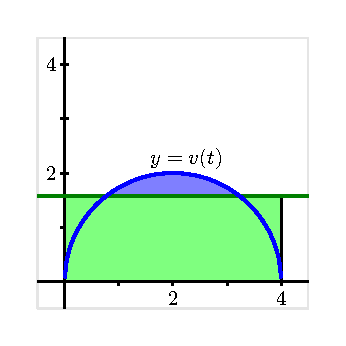
\includegraphics{figures/4_3_Act3Soln.eps}
	\end{center}
	The height of the rectangle is the average value of $v$, specifically $v_{\mbox{\tiny{AVG}}}[0,4] = \frac{\pi}{2} \approx 1.57$.
	\item Knowing that average velocity is $\frac{\pi}{2}$, it follows from the fact that distance traveled equals average rate times time (provided velocity is always nonnegative), we have
	$$D = \frac{\pi}{2} \cdot 4 = 2\pi.$$
	We see from (c) or (f) that we are simply considering the situation from two different perspectives: if we know the distance traveled, we can find average velocity, or if we know average velocity, we can find distance traveled.
\ea
\end{activitySolution}
\aftera







%----------------------------------------------------------------------------
% SUBSECTION THE MEAN VALUE THEOREM FOR INTEGRALS
%----------------------------------------------------------------------------
\subsection*{The Mean Value Theorem for Integrals}

The average value of a function brings us to an important theoretical result.  The Mean Value Theorem for Integrals says that if $f$ is continuous on the interval $[a,b]$, then there is at least one point $c$ in the interval $[a,b]$ such that $f(c)$ equals the average value of $f$ on $[a,b]$.  In other words, the horizontal line $y = f_{\mbox{\tiny{AVG}}[a,b]}$ intersects the graph of $f$ for some point $c$ in $[a,b]$, or over the interval $[a,b]$, the average value of a function $f$ must equal its actual value at least once.\footnote{Compare this statement to the Mean Value Theorem for Derivatives, which says that over the interval $[a,b]$ the instantaneous rate of change of some function must equal its average rate of change at least once.}

\concept{Mean Value Theorem for Integrals}
{Let $f$  be continuous on the interval $[a,b]$.  There exists a point $c$ in $[a,b]$ such that
\[ f(c) = \frac{1}{b-a} \int_a^b f(x) \ dx. \]
}

\noindent\textbf{Proof:} We begin by letting $F(x) = \int_a^x f(t) \ dt$ and noting that $F$ is continuous on $[a,b]$ and differentiable on $(a,b)$ by the FTC.  We now apply the Mean Value Theorem for Derivatives to $F$ and conclude that there exists at least one point $c$ in $(a,b)$ such that
\[ F'(c) = f(c) = \frac{F(b) - F(a)}{b-a}. \]
By the FTCII, we know that $F(b) - F(a)$ equals $\int_a^b f(x) \ dx$, so we can write
\[ f(c) = \frac{1}{b-a} \int_a^b f(x) \ dx \]
where $c$ is a point in $(a,b)$. \qed

%%%%%%%%%%%%%%%%%%%%%%%%%%%%%%%%%%%%%%%%%%%%%%%%%%%%%

%%\mfigure{.8}{A graph of a function $f$ to introduce the Mean Value Theorem.}{fig:ftc7a}{figures/figftc7a} %FIGURE 5.26 IN APEX 
%
%Consider the graph of a function $f$ in Figure \ref{fig:ftc7a} and the area defined by $\int_1^4 f(x)\ dx$. Three rectangles are drawn in Figure \ref{fig:ftc7b}; in (a), the height of the rectangle is greater than $f$ on $[1,4]$, hence the area of this rectangle is is greater than $\int_0^4 f(x)\ dx$. 
%
%In (b), the height of the rectangle is smaller than $f$ on $[1,4]$, hence the area of this rectangle is less than $\int_1^4 f(x)\ dx$.
%
%%\mtable{.4}{Differently sized rectangles give upper and lower bounds on $\int_1^4 f(x)\ dx$; the last rectangle matches the area exactly.}{fig:ftc7b} %FIGURE 5.27 IN APEX
%
%Finally, in (c) the height of the rectangle is such that the area of the rectangle is \textit{exactly} that of $\int_0^4 f(x)\ dx$. Since rectangles that are ``too big'', as in (a), and rectangles that are ``too little,'' as in (b), give areas greater/lesser than $\int_1^4 f(x)\ dx$, it makes sense that there is a rectangle, whose top intersects $f(x)$ somewhere on $[1,4]$, whose area is \textit{exactly} that of the definite integral.
%
%We state this idea formally in a theorem.
%
%\concept{The Mean Value Theorem of Integration} % CONCEPT
%{Let $f$ be continuous on $[a,b]$.
%\index{Mean Value Theorem!of integration}\index{integration!Mean Value Theorem}
%There exists a value $c$ in $[a,b]$ such that $$\int_a^bf(x)\ dx = f(c)(b-a).$$
%} % end concept
%
%This is an \emph{existential} statement; $c$ exists, but we do not provide a method of finding it. Theorem \ref{thm:mvt2} is directly connected to the Mean Value Theorem of Differentiation, given as Theorem \ref{thm:mvt}; we leave it to the reader to see how.  %check labels for ref
%
%We demonstrate the principles involved in this version of the Mean Value Theorem in the following example.
%
%%%\begin{marginfigure} % MARGIN FIGURE
%\margingraphics{figures/figftc8}
%\caption{A graph of $y=\sin x$ on $[0,\pi]$ and the rectangle guaranteed by the Mean Value Theorem.}
%\end{marginfigure}

\begin{example}  % EXAMPLE 
Consider $\int_0^\pi \sin x\ dx$. Find a value $c$ guaranteed by the Mean Value Theorem.

\solution We first need to evaluate $\int_0^\pi \sin x\ dx$. (This was previously done in Example \ref{ex_ftc4}.)
\[ \int_0^\pi\sin x\ dx =	-\cos x \Big|_0^\pi = 2. \]
Thus we seek a value $c$ in $[0,\pi]$ such that $\pi\sin c =2$. 
\[ \pi\sin c = 2\ \ \Rightarrow\ \ \sin c = 2/\pi\ \ \Rightarrow\ \ c = \arcsin(2/\pi) \approx 0.69. \]
In Figure \ref{fig:ftc8} $\sin x$ is sketched along with a rectangle with height $\sin (0.69)$. The area of the rectangle is the same as the area under $\sin x$ on $[0,\pi]$.
\end{example} % EXAMPLE
%
%Let $f$ be a function on $[a,b]$ with $c$ such that $f(c)(b-a) = \int_a^bf(x)\ dx$. Consider $\int_a^b\big(f(x)-f(c)\big)\ dx$:
%\begin{align*}
%\int_a^b\big(f(x)-f(c)\big)\ dx &=	\int_a^b f(x) - \int_a^b f(c)\ dx\\
%&= f(c)(b-a) - f(c)(b-a) \\
%&= 0.
%\end{align*}
%When $f(x)$ is shifted by $-f(c)$, the amount of area under $f$ above the $x$--axis on $[a,b]$ is the same as the amount of area below the $x$--axis above $f$; see Figure \ref{fig:ftc9} for an illustration of this. In this sense, we can say that $f(c)$ is the \textit{average value} of $f$ on $[a,b]$. 
%
%%\mtable{.45}{On top, a graph of $y=f(x)$ and the rectangle guaranteed by the Mean Value Theorem. Below, $y=f(x)$ is shifted down by $f(c)$; the resulting ``area under the curve'' is 0.}{fig:ftc9}
%%{\myincludegraphics{figures/figftc9a}\\ \noindent \myincludegraphics{figures/figftc9b}}
%
%The value $f(c)$ is the average value in another sense. First, recognize that the Mean Value Theorem can be rewritten as $$f(c) = \frac{1}{b-a}\int_a^b f(x)\ dx,$$ for some value of $c$ in $[a,b]$. Next, partition the interval $[a,b]$ into $n$ equally spaced subintervals, $a=x_1 < x_2 < \ldots < x_{n+1}=b$ and choose any $c_i$ in $[x_i,x_{i+1}]$. The average of the numbers $f(c_1)$, $f(c_2)$, \ldots, $f(c_n)$ is:
%\[ \frac1n\Big(f(c_1) + f(c_2) + \ldots + f(c_n)\Big) = \frac1n\sum_{i=1}^n f(c_i). \]
%Multiply this last expression by 1 in the form of $\frac{(b-a)}{(b-a)}$:
%\begin{align*}
%\frac1n\sum_{i=1}^n f(c_i) &= \sum_{i=1}^n f(c_i)\frac1n \\
%&= \sum_{i=1}^n f(c_i)\frac1n \frac{(b-a)}{(b-a)} \\
%&= \frac{1}{b-a} \sum_{i=1}^n f(c_i)\frac{b-a}n  \\
%&=\frac{1}{b-a} \sum_{i=1}^n f(c_i)\Delta x\quad \text{\scriptsize (where $\Delta x = (b-a)/n$)} % \\
%\end{align*}
%Now take the limit as $n\to\infty$:
%\[ \lim_{n\to\infty} \frac{1}{b-a} \sum_{i=1}^n f(c_i)\Delta x\quad  = \quad \frac{1}{b-a} \int_a^b f(x)\ dx\quad = \quad  f(c).\]
%This tells us this: when we evaluate $f$ at $n$ (somewhat) equally spaced points in $[a,b]$, the average value of these samples is $f(c)$ as $n\to\infty$.
%
%This leads us to a definition.
%
%\definition{The Average Value of $f$ on $[a,b]$} % DEFINITION
%{Let $f$ be continuous on $[a,b]$. The \textbf{average value of\ \ $f$\ \ on $[a,b]$} is $f(c)$, where $c$ is a value in $[a,b]$ guaranteed by the Mean Value Theorem.\index{integration!average value}\index{average value of function} I.e., 
%$$\text{Average Value of $f$ on $[a,b]$} = \frac{1}{b-a}\int_a^b f(x)\ dx.$$
%} % end definition
%
%An application of this definition is given in the following example.
%
%%\begin{example} % EXAMPLE
An object moves back and forth along a straight line with a velocity given by $v(t) = (t-1)^2$ on $[0,3]$, where $t$ is measured in seconds and $v(t)$ is measured in ft/s. 

What is the average velocity of the object?

\solution By our definition, the average velocity is:
\[ \frac{1}{3-0}\int_0^3 (t-1)^2\ dt =\frac13 \int_0^3 \big(t^2-2t+1\big)\ dt = \left.\frac13\left(\frac13t^3-t^2+t\right)\right|_0^3 = 1\text{ ft/s}. \]
\end{example} % EXAMPLE
%
%We can understand the above example through a simpler situation. Suppose you drove 100 miles in 2 hours. What was your average speed? The answer is simple: displacement/time = 100 miles/2 hours = 50 mph.
%
%What was the displacement of the object in Example \ref{ex_ftc10}? We calculate this by integrating its velocity function: $\int_0^3 (t-1)^2\ dt = 3$ ft. Its final position was 3 feet from its initial position after 3 seconds: its average velocity was 1 ft/s.
%
%%\input{activities/ }

%--------------------------------------------
% SUBSECTION INTEGRATION 
%--------------------------------------------

\begin{summary}
\item The definite integral $\int_a^b f(x) \,dx$ measures the exact net signed area bounded by $f$ and the horizontal axis on $[a,b]$; in addition, the value of the definite integral is related to what we call the average value of the function on $[a,b]$: $f_{\mbox{\tiny{AVG}}[a,b]} = \frac{1}{b-a} \cdot \int_a^b f(x) \, dx.$  

\item To find the area between two curves, we think about slicing the region into thin rectangles.  If, for instance, the area of a typical rectangle on the interval $x = a$ to $x = b$ is given by $A_{\mbox{\small{rect}}} = (g(x) - f(x)) \triangle x,$ then the exact area of the region is given by the definite integral
\[ A = \int_a^b (g(x)-f(x))\, dx. \]

\item The shape of the region usually dictates whether we should use vertical rectangles of thickness $\triangle x$ or horizontal rectangles of thickness $\triangle y$.  We desire to have the height of the rectangle governed by the difference between two curves:  if those curves are best thought of as functions of $y$, we use horizontal rectangles, whereas if those curves are best viewed as functions of $x$, we use vertical rectangles.
\end{summary}

%\begin{exercises} 
  \item Find the exact area of each described region.
  	\ba 
		\item The finite region between the curves $x = y(y-2)$ and $x=-(y-1)(y-3)$.
		\item The region between the sine and cosine functions on the interval $[\frac{\pi}{4}, \frac{3\pi}{4}]$.
		\item The finite region between $x = y^2 - y - 2$ and $y = 2x-1$.
		\item The finite region between $y = mx$ and $y = x^2-1$, where $m$ is a positive constant.
	\ea
    
   \item Let $f(x) = 1-x^2$ and $g(x) = ax^2 - a$, where $a$ is an unknown real number.  For what value(s) of $a$ is the area between the curves $f$ and $g$ equal to 2?
   
    
   \item Let $f(x) = 2-x^2$.  Recall that the average value of any continuous function $f$ on an interval $[a,b]$ is given by $\frac{1}{b-a} \int_a^b f(x) \, dx$.
   	\ba
		\item Find the average value of $f(x) = 2-x^2$ on the interval $[0,\sqrt{2}]$.  Call this value $r$.
		\item Sketch a graph of $y = f(x)$ and $y = r$.  Find their intersection point(s).
		\item Show that on the interval $[0,\sqrt{2}]$, the amount of area that lies below $y = f(x)$ and above $y = r$ is equal to the amount of area that lies below $y = r$ and above $y = f(x)$.
		\item Will the result of (c) be true for any continuous function and its average value on any interval?  Why?
	\ea
   
\end{exercises}
\afterexercises
 

\cleardoublepage